\chapter{Introduction}
\label{ch:intro}

This chapter of my thesis will explain the containerization software tool Docker and the motivation behind my decision to develop a three-part software tool built to help and encourage people within Computer Science, both on an introductory level as well as those with years of experience to learn this emerging technology. It will also illustrate several issues with preexisting technologies surrounding Docker, including Docker itself, which could be improved upon allowing for an overall better experience for users of Docker and these technologies. The overall goal of this project is to develop a software which will hopefully allow for Docker and containerization to become a more widely understood tool and is explained in further detail within this section.

\break

% -- Virtual Machines (articles that talk about them) -> industry standard moving away from that- why? what are the differences between it and VMs?

\section{Docker}
\label{sec:docker}

Docker \cite{dockerDocs} is one of the industry-leading open-source containerization platforms and which allows for the development and deployment of software, tools, and more. This 'container' that Docker uses is essentially a small Virtual Machine that is the perfect size for the code being run in it and includes all of the requirements for that particular code to run smoothly and correctly. However, it is important to not treat Docker containers like Virtual Machines. This is because Virtual Machines operate next to the host operating system with the applications running separately from the host OS as can be seen in the image below.

Another important distinction which needs to be made is the difference between an image and a container. Simply, an image is just a group of files, but a container is the run time of those files. Another way to look at it is the image is the system files, like libraries, dependencies, and source code. These files contain information in a static state that cannot be changed without rebuilding the image. A container, on the other hand, is a run time based on an image. When a container starts its initial state is the conditions listed in the image. This state can then be modified and used in the container, but these changes only exist within the container and will not be present within the image. This allows for a container to be reset back to its initial state at any time simply by rebuilding that container with the image its based upon.

\begin{figure}[h!]
    \centering
    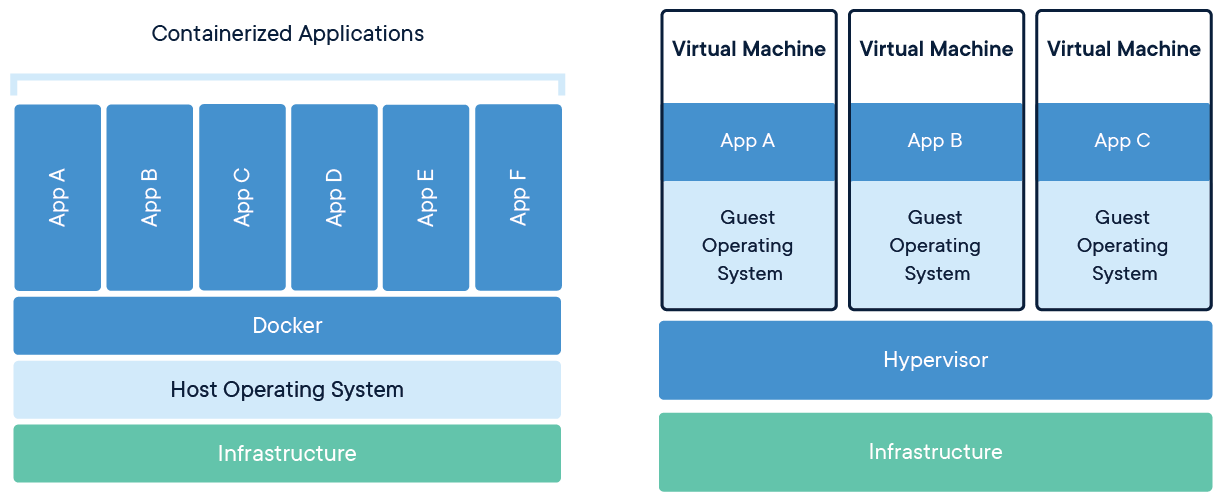
\includegraphics[width=5in]{images/Docker1}
    \caption{Virtual Machine vs Docker Container}
    \cite{dockerContainer}
\end{figure}

Docker, on the other hand, operates on top of the host OS, with applications working in tandem within the Docker platform. Another aspect of containers is that they are isolated from the host operating system and other containers and can only communicate through certain channels. An advantage that this isolation brings with it is that the container and the code stored inside are not dependent on the host OS meaning that the only requirements to run the code stored within the container are Docker and the name of the image or container. This, in a way fixes, the timeless joke of "Well, it works on my machine" by essentially allowing for a developer to ship the machine that the code was developed on.

Docker has other inherent advantages over using Virtual Machines mainly in the region of overall performance and resource use. In tests performed by MinSu Chae \cite{chae2019performance} it was found that Docker containers on a single machine outperform Virtual Machines, specifically KVM Virtual Machines in all tests that were performed by a large margin of between 3.6 to 4.6 percent. These tests focused on memory usage and CPU idle rates with at the lowest a single Docker container or Virtual Machine and highest four Docker containers or Virtual Machines. The results from these tests show the reason why the use of containerization software and platforms is slowly becoming the industry standard and the use of Virtual Machines is slowly decreasing.

There are countless other aspects of Docker from deploying a cluster of containers known as a 'swarm'. This utility can be used to ensure that a website can properly handle an increase in site traffic or have different services handled by different containers. This allows for containers to be specialized for certain tasks. This ability is also found in other tools, the most well-known one being Kubernetes which will be discussed in the Current State of the Art section \ref{sec:stateofart}.

\section{Motivation}
\label{sec:motivation}

Several events motivated me to try and create this tool as well as to become more proficient with Docker. This is an investigation based on innate curiosity and the desire to learn a new skill, as there has been a fair amount of 'buzz' within Computer Science surrounding containers and the containerization of software and software systems for a fair amount of time. However, the main push which cast me into the world of Docker was from John Abbott who is a close family friend that works for IBM and has been an on-again, off-again mentor to me. John highly suggested that I begin to look into and if possible become proficient with Docker. The reasoning behind this was from his perspective in the Computer Science industry there is a lot of movement towards containerization. Due to this, being able to demonstrate that I have some kind of rudimentary understanding and experience with Docker could make my resume more attractive to prospective employers once I began looking for a job.

This event occurred over the summer and for a short while I began to look into Docker, as well as a few other things which he suggested I take a look at but do not have any relevance. However, I quickly lost motivation due to working long days and as a result learning, Docker quickly slipped out of my mind. Once the semester began, motivation once again came, this time in the form of having to help first-year students, as well as upperclassmen, try to get Docker installed and running on their laptops. The difficulties that many of the students faced in trying to Docker to work as well as trying to figure out the differences between the version of Docker pushed me to learn as much as possible about Docker. From there I began to experiment with Docker, following the online tutorials on Docker's 'Get Started' pages to learn the basics and slowly built my understanding of how Docker worked. Eventually, I was able to make my images of incredibly simple Python programs that could receive user input or command-line arguments.

Through this process of learning the basics of Docker, I saw just how useful of a tool it can be and began to see many of the other spots where it was lacking. One of these areas was helping new users to learn the basics of Docker. The documentation online while helpful was at times overly complex and the amount of information given is not entirely necessary. This motivated me to begin to look into ways that could streamline the installation process of Docker across operating systems and create a simple interface for new users of Docker. As such, I began to look into the feasibility of such a task. In the process of exploring this, I began to wonder about automatically generating Dockerfiles. This was an area that could be incredibly useful so I tried to see if that was something that already existed and if not if it would be possible to do. After researching the feasibility of adding that component I decided that it would be and added it to the overall project.


\section{Current State of the Art}
\label{sec:stateofart}

Containerization software is slowly making its way into more and more areas in the Computer Science industry. There are many different containerization software that exists with Docker being the most well known and one of the most widely utilized. Another state of the art containerization platform that exists is Kubernetes \cite{kubernetes}, which has compatibility with some aspects of Docker and as such can be easily used interchangeably with Docker. Kubernetes has the advantage of being originally developed by Google and as such has some integrations with other Google services, like their cloud platform. Another well-known software is Microsoft's Azure \cite{azure}. This software, which is developed and maintained by Microsoft and is built off of Kubernetes. Kubernetes, while being a containerization platform acts more so as a distribution and management platform for containers as well as for coordinating clusters of Docker nodes.

\section{Goals of the Project}
\label{sec:goals}

There are several goals for this project. The first, and in my opinion, the most important goal is to gain a better understanding of Docker and how it works and can be utilized. This as previously discussed in the motivation \ref{sec:motivation} was the primary goal of looking into Docker over the summer and continues to be one of the main goals. The area of Docker and containerization is still fairly young and as such new uses and information on this topic are constantly being figured out. Due to this, there will always be something new to learn in this area, which is something that will force me to constantly learn. Being able to create Docker containers that can perform different services and run the software will hopefully reflect well in the future and as such may help in getting a job in the future.

The first tangible goal of the project is to develop a software tool that can detect the host machine's operating system and in the case of Windows and Linux the version of the OS. This will then allow for the tool to determine what the proper method to install Docker is and perform that operation. The aim of this is to allow for an easier and more streamlined installation process that can be used more universally. This as previously mentioned is due to the challenges that were faced when the Computer Science Department began to transition to the use of Docker and Docker containers in Computer Science classes.

The next goal is to develop a simple, but optimized, graphical user interface that will allow users who have no experience with Docker to learn the many command-line arguments that Docker has. Docker has forty base commands with purposes ranging from the building and creation of Docker images to removing images and containers from a given machine, which are two separate commands. Most of these forty commands are not required for an introductory user of Docker and as such can just cause further confusion with a topic that can already be intimidating when starting.

The final goal is to create a system that can be supplied with a directory that contains programs that a user wants to contain in a Docker container. This system will then determine what languages are being used and add the necessary installation commands to a Dockerfile along with adding all programs contained within the specified directory. In the end, this will create the perfect Docker container which the user can run to interact with or run the programs in the given directory.

\section{Thesis Outline}
\label{sec:outline}

The creation of this proposed tool will streamline the installation and use of Docker. Docker is an incredibly useful tool that is slowly beginning to enter more and more regions of computer science, from software to websites and web applications. As such becoming proficient with or at least having a basic understanding of how to use and utilize Docker can be a knowledge set that will be more and more useful as time goes on. The simplistic and streamlined nature of the user interface that will be proposed, will allow for introductory users of Docker to learn the basics of Docker easier. This will be due to the consolidation of the extensive command and argument list that is present in the command line operation of Docker. The proposed tool will also make it easier for the user to learn how to create Dockerfiles, which are integral to the creation and use of Docker images which are utilized by Docker containers. This aspect will be accomplished by allowing users to automatically create the Dockerfiles necessary for a given directory and learn the general structure that Dockerfiles have. The combination of these three elements of the tool, the installer, the interface, and the Dockerfile generator, will create an overall software tool that will allow a new user of Docker to more easily learn the basics.
